Los modelos matemáticos aplicados a proyectos de manipuladores robóticos son usados principalmente para realizar cálculos relacionados con los aspectos cinemáticos y dinámicos de los mismos.

Los aspectos cinemáticos de un manipulador robótico describen cómo es el movimiento y las trayectorias del mismo sin tener en cuenta las fuerzas que lo afectan, mientras que los aspectos dinámicos describen cómo se ve afectado dicho movimiento en función de las fuerzas que actúan sobre el.

Ambos aspectos anteriormente mencionados deben de ser descritos mediante un modelo matemático que permita realizar cálculos sobre los movimientos del manipulador. 

En este proyecto, se ha llevado a cabo únicamente el modelo cinemático, dado que debido a las características físicas del prototipo a construir, es decir, velocidades de desplazamiento, peso de las articulaciones o masa máxima de carga; se ha concluido que el modelo dinámico no aportaría demasiada información útil para llevar a cabo el control del manipulador. Cabe destacar que el modelo dinámico suele presentar una complejidad mucho mas elevada que el modelo cinemático en términos matemáticos y por ello se ha desechado la posibilidad de llevarlo a cabo.

Desde un punto de vista técnico, el modelo cinemático de un manipulador robótico expresa cuál es la posición del extremo del mismo con respecto al tiempo y en función de la posición de las articulaciones del mismo. Normalmente, los brazos robóticos se pueden describir matemáticamente mediante el concepto de cadena cinemática:

\begin{figure}[ht!]
    \centering 
    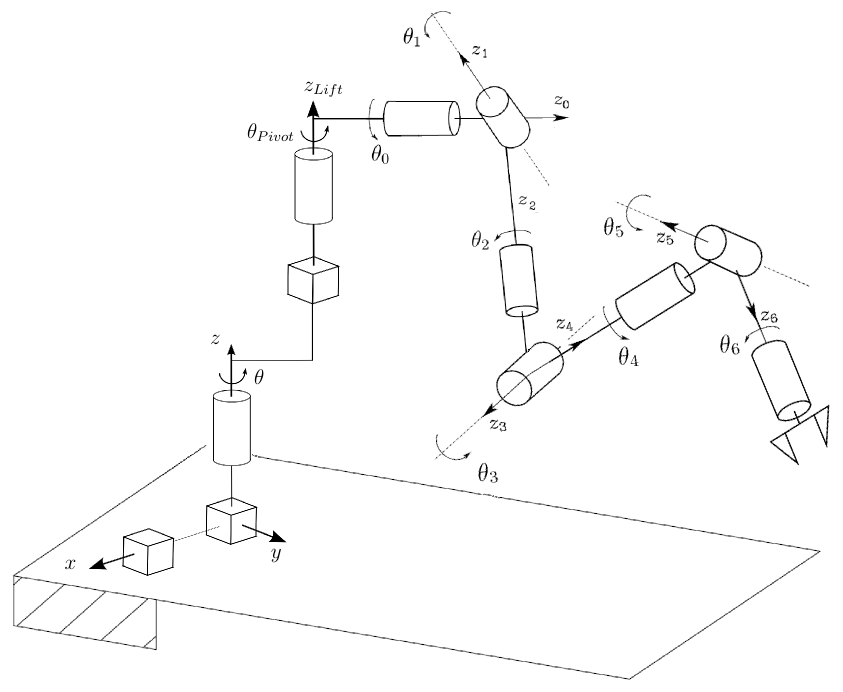
\includegraphics[width=.6\linewidth]{pictures/kinematic chain.png}
    \caption{Ejemplo de cadena cinemática \cite{noauthor_figure_nodate}.}
    \label{fig:chains}
\end{figure}

Tal y como se puede apreciar en la figura \ref{fig:chains}, las articulaciones pueden rotar y permiten la movilidad de cada uno de los segmentos del manipulador. Dado que estas articulaciones rotan, su posición se expresa numéricamente mediante unidades angulares. El concepto de cadena cinemática hace referencia a que, dado que cada una de las articulaciones esta unida a la siguiente mediante un segmento, se genera una cadena de movimientos en la que la posición espacial de cada una de las articulaciones se ve afectada por la posición angular de las anteriores.

Aplicando este principio, el modelo cinemático expresa matemáticamente la posición cartesiana del extremo del robot en función de las coordenadas angulares de las articulaciones. Existen pues dos perspectivas del modelo cinemático:

\begin{itemize}
    \item El modelo de cinemática directa expresa la posición espacial del extremo del manipulador en función de las coordenadas angulares de las articulaciones.
    \item El modelo de cinemática inversa expresa las coordenadas angulares de las articulaciones en función de las coordenadas cartesianas del extremo del manipulador.
\end{itemize}

\begin{figure}[H]
    \centering 
    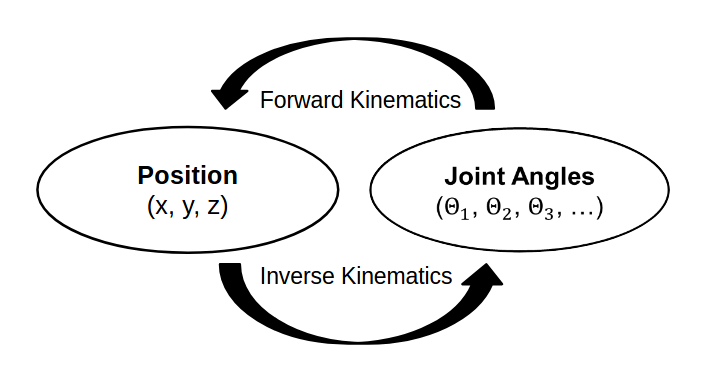
\includegraphics[width=.6\linewidth]{pictures/Kinematic Diagram.png}
    \caption{Diagrama del modelo cinemático \cite{noauthor_roboy_nodate}.}
    \label{fig:kdiagram}
\end{figure}

En conclusión, el modelo matemático conforma la base teórica y formal que permite realizar el estudio de los movimientos del manipulador y es por ello que representa un bloque crucial dentro del proyecto.


